\section{Assessment of Pain}
Pain is described as a complex and subjective experience that poses a number of measurement challenges due to its subjective nature. Nevertheless, pain measurements are necessary for pain studies as well as the evaluation of methods to control pain.~\cite{Jensen2001}
There is no valid and reliable method of objectively quantifying pain at the moment. However, despite the challenges that pain measurement present, several tools and approaches can be employed in order to collect useful pain estimates.~\cite{Younger2010} The aim of pain assessment is to diagnose the cause, understand the impact, identify appropriate pain relief strategies and evaluate their effectiveness~\cite{Briggs2010}. There are different dimensions of pain experience that can be assessed: pain intensity, pain affect, pain quality and pain location. The two types of pain assessments pain are Self-reported Scales and Psychological Methods. 

\subsection{Self-reported Scales}
Pain cannot be registered directly by clinicians, why patient self-report is frequently used to asses the experiences of pain. Within this category it is possible to apply unidimensional and multidimensional scales.~\cite{Jensen2001}

\subsubsection{Unidimensional scales}
Unidimensional scales explore only one dimension of pain. The most common assessed dimension of pain is intensity. This could be due to the fact that patients are usually able to provide quantitative pain intensity relatively rapidly.~\cite{Jensen2001}

One commonly used unidimensional tool is the Verbal Rating Scales (VRS) which consists of a list of adjectives describing different levels of pain intensity, as illustrated on \figref{fig:VRS}. This type of scales are easy to administer, score and apprehend. However, it has several statistical disadvantages and criticism raised due to the fact that assumes equal intervals between adjective.~\cite{Jensen2001}. For this particular reasons along with others it is used when the patient's conditions require it~\cite{Jensen1986}. 


\begin{figure}
\begin{subfigure}{0.8\textwidth}
  \centering
  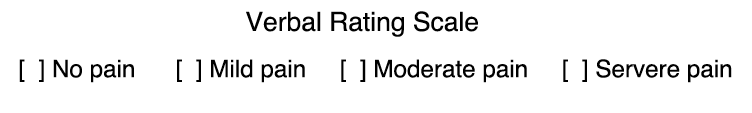
\includegraphics[width=0.8\linewidth]{figures/VRS.png}
  \caption{Verbal Rating Scales (VRS)}
  \label{fig:VRS}
\end{subfigure} \\
\begin{subfigure}{0.8\textwidth}
  \centering
  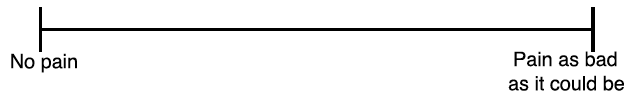
\includegraphics[width=0.8\linewidth]{figures/VAS.png}
  \caption{Visual Analogue Scales (VAS)}
  \label{fig:VAS}
\end{subfigure} \\
\begin{subfigure}{0.8\textwidth}
  \centering
  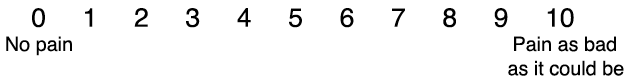
\includegraphics[width=0.8\linewidth]{figures/NRS.png}
  \caption{Numerical Rating Scales (NRS)}
  \label{fig:NRS}
\end{subfigure}
\caption{Different types of unidimensional scales}
\label{fig:fig}
\end{figure}


Other possibility of unidimensional scales is a visual analogue scale (VAS). VAS consists of a 10 cm line, as shown in \figref{fig:VAS},the ends of this line are labeled as the extremes of pain. The scale is scored by measuring the distance from 'no pain' end to the patient's mark. This fact makes the VAS more sensitive to changes in pain intensity. However, one of the drawbacks is that scoring time is higher than for other methods. 

Numerical Rating Scale (NRS), which is illustrated on \figref{fig:NRS}, is also within unidimensional tools of pain intensity measure. NRS consits of an numerical scale from 0 to 10, being described 0 as 'no pain' and  10 equal to 'higest level of pain'. The advantage of NRS is that it not requires patients mobility because the response is given verbally. NRS is a valid method and demonstrate positive and significant correlations with other measures of pain intensity \cite{Jensen1986}. 

Another method is to use pictures or face scales to illustrate facial expressions of different intensities of pain. Even though the primary purpose of this scales were to offer individuals with written language or cognitive difficulties an option to express pain intensity, there is evidence that they are valid methods \cite{Jensen2001}. 

\subsubsection{Multidimensional scales}\fxnote{Be aware that there are many different questionnaires designed for general pain, different aspects of pain, or various pain conditions.}

Multidimensional scales are convenient in relentless pain conditions. Multidimensional scales measure several dimensions of pain with different combinations of these dimensions. These scales offer a more detailed reflection of the patient's pain experience \cite{Briggs2010}. 

Within this category the McGill Pain Questionnaire (MPQ) is used. This method consists of 78 words that describe the pain in sensory, affective and evaluative terms. These tems are arranged in groups acoording to the quality of pain and intensity of this pain. A 6-point VRS is used to determ the intensity of the pain. The MPQ is proved as a valid method support by several studies.  One disadvantage of the MPQ is the length and complexity, why a brief form of this questionnaire has been introduced, the short-form McGill Pain Questionnaire (SF-MPQ)~\cite{Katz2001}. \fxnote{15 different descriptors in sensory and affective terms. Each descriptor is rated on a 4-point VRS scale.}

Another scale, breif pain inventory (BPI), was developed to assess cancer pain and have been proven as a useful instrument to asses different kinds of pain in several clinical settings. The BPI measures pain severity, pain quality and the disturbance caused in the patients daily life. Two subscale scores pain intensity and pain interference~\cite{Katz2001}.  

\subsection{Psychological methods}
Quantitative sensory testing (QST) evaluates the integrity of the entire sensory neuraxis receptor to the cortex. Even though QST has recieved criticism for being subjective, it is a reliable test. Brain imaging studies provided evidence that subjective pain magnitude scores are associated with objectively measured neural activity in areas of the brain involved in pain processing. QST include different modalities of stimulation, such as thermal, mechanical, electrical, ischemic and chemical. This method provide two different assessments of pain. On the one hand the  evaluation of endogenous pain, which is the pain that the patient experiences due to the disease process. On the other hand, the assessment of induced pain, in order to experiment on pain mechanisms or therapy. \cite{Yarnitsky2006}

\subsubsection{Measurement of experimental pain} \fxnote{How would you link 'measurement of experimental pain' to 'psychological methods of pain assessment'?}
As a result to a set of experimental noxious stimuli, it is possible to obtain different parameters such as, pain thresholds, tolerance or suprathreshold pain intensities. Threshold is defined as the stimulus that produces an arbitrary, but defined, level of performance. There is a distinction between receptor or absolute threshold and psychophysical or sensory threshold. Absolute threshold is the energy required to elicit response in the primary afferent while the psychophysical or sensory threshold, is the minimal energy necessary to reach perception. Due to the fact that receptor threshold is lower than sensory threshold, the sensory threshold is a convenient parameter which offers the transition point between non-painful and painful stimulus. \cite{Yarnitsky2006}

\subsubsection{Psychophysical Procedure} \fxnote{what is the difference between 'psychophysical methods' and 'psychophysical procedure'?}
Psychophysical research has been mostly concentrated on thresholds measurement owing to, the desire to isolate low-level sensory mechanisms using operationally defined tasks that are intended to minimize the roles of perception and cognition \cite{Pelli2010}. There are different procedures in order to measure thresholds, such as methods of adjustment, methods of limits, methods of constant stimuli, adaptive or staircase procedure and forced-choice performance procedures. 

%Performance-Based Procedures 
%Appearance-Based Procedures

\textbf{Methods of adjustment}
\\
The test subject adjust the magnitude of a stimulus, until a prespecified criterion is reached. This method is commonly used for appearance-based tasks. Currently, this method is not commonly used to obtain performance measures, due to the fact that forced-choice procedures are consider superior. However, the method of adjustment is useful for obtaining a rough threshold estimate to guide the choice of stimulus magnitudes for a forced-choice procedure, when there are different conditions to be measured.

\textbf{Forced-choice Performance Procedures}
\\
The forced-choice tasks can be termed by Alternative Forced-Choice (AFC) or Interval Forced-Choice (IFC). In IFC procedures the stimulus are presented in temporal order. There are different varieties within forced-choice performance procedures. AFC using two stimuli in each trial are the most popular in psychophysics. One of the stimuli is the target, which is selected by the test subjects.


\textbf{Methods of limits} 
\\
In this method, different magnitude stimuli are presented to the test subject, in ascending or descending order. The subject indicates whether or not the stimulus are detected on each presentation. Accordingly, the threshold in each case is the stimulus magnitude at which the response switches from non perception to perception and/or vice versa. The patient's response cannot be evaluated if it is correct or incorrect. \cite{Kingdom2016}.

*** SHORT THE SECTION UNDER: ****


%One of the drawbacks of this method is that the observer may get used to reporting that is perceiving a stimulus or not. As a result, he or she continues to give the same response even at stimulus magnitudes that are higher or lower than the threshold. This phenomena is the error of habituation. Contrarily, the observer may anticipate the response and make a premature judgment, which is call the error of expectation. Another disadvantages using this method is that the parameter value from perception to non-perception differ from non-perception to perception value, due to different artifacts \cite{Hock2010}.

\textbf{Method of constant stimuli}
\\
The stimulus magnitude on each trial is randomly selected from a predefined set. This range is selected to straddle the threshold value. This method generates data, when this data fitted with the appropriate psychometric function, provides the most accurate estimates of the threshold. The choice of this stimulus set sometimes demand pilot work to obtain an estimate of the threshold. The method of adjustment, as explained before, can be useful for this purpose. It is possible to use this method simultaneously with appearance-based procedures. The selection of the stimuli range is crucial. In order to avoid the problem of selecting an incorrect set, an adaptive or staircase procedure is apply.

\textbf{Adaptive or staircase procedure}
\\
An algorithm, that analyzes the previous trials response, selects the stimulus magnitude on each trial. This method can be used simultaneously  with conventional methods as well as with performance-based and appearance-based tasks.

